\documentclass{tufte-handout}

\title{3.1 Quadratic functions and models}

\author[AW]{Ammon Washburn}

\usepackage{graphicx} % allow embedded images
  \setkeys{Gin}{width=\linewidth,totalheight=\textheight,keepaspectratio}
  \graphicspath{{graphics/}} % set of paths to search for images
\usepackage{amsmath}  % extended mathematics
\usepackage{booktabs} % book-quality tables
\usepackage{units}    % non-stacked fractions and better unit spacing
\usepackage{multicol} % multiple column layout facilities
\usepackage{lipsum}   % filler text
\usepackage[inline]{enumitem}
\usepackage{fancyvrb} % extended verbatim environments
  \fvset{fontsize=\normalsize}% default font size for fancy-verbatim environments

% Standardize command font styles and environments
\newcommand{\doccmd}[1]{\texttt{\textbackslash#1}}% command name -- adds backslash automatically
\newcommand{\docopt}[1]{\ensuremath{\langle}\textrm{\textit{#1}}\ensuremath{\rangle}}% optional command argument
\newcommand{\docarg}[1]{\textrm{\textit{#1}}}% (required) command argument
\newcommand{\docenv}[1]{\textsf{#1}}% environment name
\newcommand{\docpkg}[1]{\texttt{#1}}% package name
\newcommand{\doccls}[1]{\texttt{#1}}% document class name
\newcommand{\docclsopt}[1]{\texttt{#1}}% document class option name
\newenvironment{docspec}{\begin{quote}\noindent}{\end{quote}}% command specification environment

\newtheorem{mydef}{Definition}
\providecommand{\floor}[1]{\left \lfloor #1 \right \rfloor }

\begin{document}
\maketitle

\begin{abstract}
Learn how to figure out the properties of quadratic equations and use them in models
\end{abstract}

\section{Polynomials}

\begin{mydef}
A polynomial is an equation of the form $p(x) = a_n x^n + a_{n-1} x^{n-1} + \cdots + a_1 x + a_0$ where $a_n \neq 0$.
\end{mydef}

The degree of the polynomial is the highest power of $x$ in the equation.

\begin{itemize}
\item A zero degree polynomial is $p(x) = a_0$
\item A first degree polynomial or line is $p(x) = a_1 x + a_0$
\item A second degree polynomial or a quadratic function is $p(x) = a_2 x^2 + a_1 x + a_0$
\end{itemize}

\subsection{Quadratic Functions}
The graph of a quadratic function is called a parabola.  Essentially it is the function $q(x) = x^2$ that has been transformed.  It is not easy to see in the form above but you can see it in other forms.

\begin{mydef}
The standard form of a quadratic function is when it looks like this: $t(x) = a(x-h)^2 + k$.
\end{mydef}

This is normally called vertex form because the vertex is easy to see but the textbook calls it standard form.  What is the vertical stretch? What is the horizontal shift? What is the vertical shift? Are we shifting first or doing our stretching?

We can always write an equation in the general form from before into standard form.  The easiest way for me? Use completing the square.  However, most students don't like completing the square so I will teach you another way (which is exactly like completing the square only slower).

Say you have an equation in the following form:
\[
p(x) = ax^2 + bx +c
\]
Then you can see that $a=a$ and we can prove (using completing the square) that $h = -\frac{b}{2a}$.  Then we can plug in a point from above (Easiest point is $(0,c)$) and then solve for k.  Then you can see that $k = c-\frac{b^2}{4a}$.

\noindent \textbf{Example:}

Put $f(x) = 3x^2 + 24 x - 20$ in standard form.  Answer: Standard form is $f(x) = 3(x + 4)^2  - 68$. What is the vertex?

You can check using the table function of your calculator. Show table to students.

\subsection{Max and Min values of Quadratic Function}

The vertex is a special point.  It represents either the minimum or maximum of a quadratic function.  The $a$ in standard form represents the stretch and if there is reflection over x-axis.  Whether $a>0$ or $a<0$ will tell you if the quadratic has a max or min.

\begin{mydef}
A quadratic function $f(x) = a (x-h)^2 + k$ has attains a minimum $k$ at $x = h$ when $a>0$. Conversely $f(x)$ attains a maximum $k$ at $x=h$ when $a<0$.
\end{mydef}

Is $h$ a maximum or minimum? No, it is WHERE the function attains the maximum and minimum.

Using this information we can also find the range of any quadratic function.

\subsection{Applications with Quadratic Functions}

Consider having the students find the equation below for warm-up problem. Note that the equation is wrong and should be $A(n) = (700+n)(10-0.1n)$.

\begin{figure}
\centering
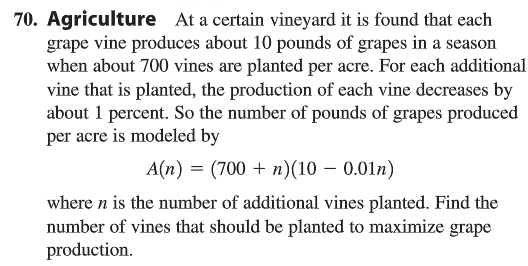
\includegraphics[width = \linewidth]{3-1QuadApp.png}
\end{figure}



\end{document}